% ULTRA paper: IEEE two-column conference format. Main file: paper.tex -> paper.pdf (committed).
% Build: `just paper` from the repository root (regenerates data/metrics.tex, runs
% pdflatex + bibtex + pdflatex x2, and fails on undefined references or citations).
% Every result number comes from data/metrics.tex (generated by python/ultra/tools/paper_data.py).
% Sections must not contain literal result numbers; missing metrics print a red "??" via \PH.
\documentclass[conference]{IEEEtran}
\IEEEoverridecommandlockouts

\usepackage[T1]{fontenc}
\usepackage{lmodern}
\usepackage{amsmath,amssymb}
\usepackage{graphicx}
\usepackage[table]{xcolor}
\usepackage{booktabs}
\usepackage{multirow}
\usepackage{tikz}
\usepackage{pgfplots}
\pgfplotsset{compat=1.17}
\usetikzlibrary{arrows.meta,positioning,calc,fit,backgrounds,patterns}
\usepgfplotslibrary{groupplots,fillbetween}
\usepackage{xspace}
\usepackage{microtype}
\usepackage{cite}
\usepackage{flushend}% balance the columns of the last page
\usepackage{url}
\usepackage[hidelinks]{hyperref}
\usepackage[capitalise,nameinlink]{cleveref}
\usepackage[firstpage=false,stamp=true]{draftwatermark}
\SetWatermarkText{PRELIMINARY}
\SetWatermarkScale{0.9}
\SetWatermarkColor[gray]{0.955}

% ---------------------------------------------------------------- placeholders and metrics
\definecolor{phred}{RGB}{200,0,0}
% \PH{name}: a metric that data/metrics.tex does not define yet. Prints a red "??".
\newcommand{\PH}[1]{\textcolor{phred}{\textbf{??}}\ifmmode\else\fi}
\IfFileExists{data/metrics.tex}{% Generated by python/ultra/tools/paper_data.py. Do not edit by hand.
% Every macro is a bare number (no unit, no %). Provenance: docs/paper/data/SOURCES.md.
% Labels: exploratory = shared-host / non-qualifying measurement; reported = configuration
% or descriptive constant; qualified = from a qualifying window (none yet).
\providecommand{\PaperMissing}[1]{\textcolor{red}{??}}

\newcommand{\AASpread}{25}% [exploratory] % CPU
\newcommand{\AbabBlocks}{8}% [reported] blocks
\newcommand{\AbabPholmDense}{\ensuremath{1.4\times10^{-10}}}% [exploratory] p
\newcommand{\AbabPholmMR}{\ensuremath{1.9\times10^{-6}}}% [exploratory] p
\newcommand{\AbabRatioDense}{0.666}% [exploratory] x
\newcommand{\AbabRatioDenseHi}{0.678}% [exploratory] x
\newcommand{\AbabRatioDenseLo}{0.655}% [exploratory] x
\newcommand{\AbabRatioMR}{0.629}% [exploratory] x
\newcommand{\AbabRatioMRHi}{0.684}% [exploratory] x
\newcommand{\AbabRatioMRLo}{0.578}% [exploratory] x
\newcommand{\AbabSpeedDense}{1.50}% [exploratory] x
\newcommand{\AbabSpeedMR}{1.59}% [exploratory] x
\newcommand{\AvgGainClean}{0.43}% [exploratory] pp WER
\newcommand{\AvgGainOther}{0.84}% [exploratory] pp WER
\newcommand{\BOneAttnCut}{3--10}% [exploratory] %
\newcommand{\BeamGainClean}{0.63}% [exploratory] pp WER
\newcommand{\BeamGainOther}{1.19}% [exploratory] pp WER
\newcommand{\BridgeStep}{5{,}000}% [reported] steps
\newcommand{\CCXCount}{16}% [reported] CCX
\newcommand{\ChunkSixteenGainClean}{0.39}% [exploratory] pp WER
\newcommand{\ChunkSixteenGainOther}{0.90}% [exploratory] pp WER
\newcommand{\ColdRowsCount}{0}% [reported] rows
\newcommand{\CoresPerCCX}{4}% [reported] cores
\newcommand{\CostClaimDense}{0.0369}% [exploratory] CPU-s/audio-s
\newcommand{\CostClaimMR}{0.0279}% [exploratory] CPU-s/audio-s
\newcommand{\CostClaimRzero}{0.0864}% [exploratory] CPU-s/audio-s
\newcommand{\CostEngineFP}{0.104}% [exploratory] CPU-s/audio-s
\newcommand{\CostEngineIntEight}{0.041}% [exploratory] CPU-s/audio-s
\newcommand{\CostLadderDense}{0.0443}% [exploratory] CPU-s/audio-s
\newcommand{\CostLadderMR}{0.0354}% [exploratory] CPU-s/audio-s
\newcommand{\CostLadderRzero}{0.0864}% [exploratory] CPU-s/audio-s
\newcommand{\CostNemo}{0.472}% [exploratory] CPU-s/audio-s
\newcommand{\CostORT}{0.175}% [exploratory] CPU-s/audio-s
\newcommand{\CostRatioDense}{1.95}% [exploratory] x
\newcommand{\CostRatioMR}{2.44}% [exploratory] x
\newcommand{\CostRzero}{0.078}% [exploratory] CPU-s/audio-s
\newcommand{\DenDenseCCX}{96}% [exploratory] streams/CCX
\newcommand{\DenDenseCore}{24}% [exploratory] streams/core
\newcommand{\DenFailDenseCCX}{112}% [exploratory] streams/CCX
\newcommand{\DenFailMRCCX}{160}% [exploratory] streams/CCX
\newcommand{\DenFailRzeroCCX}{48}% [exploratory] streams/CCX
\newcommand{\DenMRCCX}{144}% [exploratory] streams/CCX
\newcommand{\DenMRCore}{36}% [exploratory] streams/core
\newcommand{\DenPninetyNineDense}{596}% [exploratory] ms
\newcommand{\DenPninetyNineMR}{735}% [exploratory] ms
\newcommand{\DenPninetyNineRzero}{729}% [exploratory] ms
\newcommand{\DenRatioDense}{3.0}% [exploratory] x
\newcommand{\DenRatioMR}{4.5}% [exploratory] x
\newcommand{\DenRatioMRvsDense}{1.5}% [exploratory] x
\newcommand{\DenRungSeconds}{20}% [reported] s
\newcommand{\DenRzeroCCX}{32}% [exploratory] streams/CCX
\newcommand{\DenRzeroCore}{8}% [exploratory] streams/core
\newcommand{\DenWorkers}{4}% [reported] workers
\newcommand{\DtwoAudioHoursRehearsal}{6303}% [reported] audio-h
\newcommand{\DtwoEpoch}{8}% [reported] epoch (0-indexed)
\newcommand{\DtwoEpochRehearsal}{6}% [reported] epoch (0-indexed)
\newcommand{\DtwoStep}{60{,}000}% [reported] steps
\newcommand{\EngineBeamMRDelta}{\ensuremath{-}1.43}% [exploratory] pp WER
\newcommand{\FrontierDense}{0.0435}% [exploratory] CPU-s/audio-s
\newcommand{\FrontierMR}{0.0330}% [exploratory] CPU-s/audio-s
\newcommand{\FrontierPerCoreDense}{23.0}% [exploratory] streams/core
\newcommand{\FrontierPerCoreMR}{30.3}% [exploratory] streams/core
\newcommand{\FrontierPerCoreRzero}{14.3}% [exploratory] streams/core
\newcommand{\FrontierRzero}{0.0698}% [exploratory] CPU-s/audio-s
\newcommand{\FrontierStreams}{16}% [reported] streams
\newcommand{\FullAttnLossClean}{0.81}% [exploratory] pp WER
\newcommand{\GateBeamDelta}{+0.007}% [exploratory] pp WER
\newcommand{\GateBeamUpper}{+0.150}% [exploratory] pp WER
\newcommand{\GateDenseDelta}{+0.021}% [exploratory] pp WER
\newcommand{\GateDenseUpper}{+0.157}% [exploratory] pp WER
\newcommand{\GateDtwoAvgDelta}{+0.042}% [exploratory] pp WER
\newcommand{\GateDtwoAvgUpper}{+0.140}% [exploratory] pp WER
\newcommand{\GateMRDelta}{+0.069}% [exploratory] pp WER
\newcommand{\GateMRUpper}{+0.203}% [exploratory] pp WER
\newcommand{\GateMargin}{0.10}% [reported] pp WER
\newcommand{\GateMaxUpper}{+0.211}% [exploratory] pp WER
\newcommand{\GemmShare}{75--80}% [exploratory] %
\newcommand{\GreedyDecoderCost}{0.0016}% [exploratory] CPU-s/audio-s
\newcommand{\IntEightMRDenCCX}{136}% [exploratory] streams/CCX
\newcommand{\IntEightUncentred}{+0.207}% [exploratory] pp WER
\newcommand{\LThreeMiB}{16}% [reported] MiB
\newcommand{\LeftSixtyFourAttn}{0.70}% [exploratory] x of 128
\newcommand{\LeftSixtyFourDelta}{+0.09}% [exploratory] pp WER
\newcommand{\LeftThirtyTwoAttn}{0.45}% [exploratory] x of 128
\newcommand{\LeftThirtyTwoDelta}{+0.68}% [exploratory] pp WER
\newcommand{\MRBeamPanelBeamFP}{14.43}% [exploratory] % WER
\newcommand{\MRBeamPanelBeamInt}{14.44}% [exploratory] % WER
\newcommand{\MRBeamPanelGreedyFP}{15.86}% [exploratory] % WER
\newcommand{\MRPadDeltaMax}{0.03}% [exploratory] pp WER
\newcommand{\MatchedRung}{32}% [reported] streams/CCX
\newcommand{\NemoLongCost}{0.451}% [exploratory] CPU-s/audio-s
\newcommand{\NemoLongTestClean}{2.58}% [exploratory] % WER
\newcommand{\NemoLongTestOther}{5.18}% [exploratory] % WER
\newcommand{\NemoShortCost}{0.709}% [exploratory] CPU-s/audio-s
\newcommand{\NemoShortTestClean}{2.65}% [exploratory] % WER
\newcommand{\NemoShortTestOther}{5.60}% [exploratory] % WER
\newcommand{\PanelSpeakers}{73}% [reported] speakers
\newcommand{\ParamsDtwo}{58.7}% [reported] M parameters
\newcommand{\ParamsDtwoMR}{59.2}% [reported] M parameters
\newcommand{\ParityFP}{\ensuremath{2.4\times10^{-6}}}% [exploratory] abs error
\newcommand{\QkvCapRatio}{1.5}% [reported] x
\newcommand{\QkvRunawayFrom}{70}% [exploratory] norm
\newcommand{\QkvRunawayTo}{684}% [exploratory] norm
\newcommand{\RssEngineFP}{478}% [exploratory] MB
\newcommand{\RssEngineIntEight}{646}% [exploratory] MB
\newcommand{\RssEngineIntEightPrepared}{259}% [reported] MB
\newcommand{\RssNemo}{1{,}284}% [exploratory] MB
\newcommand{\RssORT}{776}% [exploratory] MB
\newcommand{\RssRzero}{239}% [exploratory] MB
\newcommand{\SingleMthreeDense}{0.0132}% [exploratory] CPU-s/audio-s
\newcommand{\SingleMthreeMR}{0.0123}% [exploratory] CPU-s/audio-s
\newcommand{\SingleZenDense}{0.040}% [exploratory] CPU-s/audio-s
\newcommand{\SpeedupEngineFPVsORT}{1.7}% [exploratory] x
\newcommand{\SpeedupVsORT}{4.2}% [exploratory] x
\newcommand{\SpeedupVsRzero}{1.9}% [exploratory] x
\newcommand{\StackGainClean}{0.99}% [exploratory] pp WER
\newcommand{\StackGainOther}{2.02}% [exploratory] pp WER
\newcommand{\StreamsPerCoreMthreeMR}{84}% [exploratory] streams/core
\newcommand{\StreamsPerCoreMthreeMRFail}{96}% [exploratory] streams/core
\newcommand{\SweepDtwoBeamFourPooled}{10.82}% [exploratory] % WER
\newcommand{\SweepDtwoBestBeam}{8}% [exploratory] beam
\newcommand{\SweepDtwoBestPooled}{10.69}% [exploratory] % WER
\newcommand{\SweepDtwoGreedyPooled}{11.67}% [exploratory] % WER
\newcommand{\SweepDtwoMRBeamFourPooled}{14.41}% [exploratory] % WER
\newcommand{\SweepDtwoMRBestBeam}{8}% [exploratory] beam
\newcommand{\SweepDtwoMRBestPooled}{14.20}% [exploratory] % WER
\newcommand{\SweepDtwoMRGreedyPooled}{15.89}% [exploratory] % WER
\newcommand{\TernaryDenCCX}{112}% [exploratory] streams/CCX
\newcommand{\TernaryEngineWer}{17.98}% [exploratory] % WER
\newcommand{\TernaryMiB}{14.26}% [reported] MiB
\newcommand{\TernaryZeros}{31.8}% [reported] %
\newcommand{\TrainHours}{960}% [reported] h
\newcommand{\UsevenBar}{1.2}% [reported] x
\newcommand{\UsevenVsActHi}{0.92}% [exploratory] x
\newcommand{\UsevenVsActLo}{0.89}% [exploratory] x
\newcommand{\UsevenVsKzeroHi}{1.01}% [exploratory] x
\newcommand{\UsevenVsKzeroLo}{0.94}% [exploratory] x
\newcommand{\WerBridgeFP}{21.88}% [exploratory] % WER
\newcommand{\WerBridgeIntEight}{21.80}% [exploratory] % WER
\newcommand{\WerDtwoAvgGreedyClean}{7.22}% [exploratory] % WER
\newcommand{\WerDtwoAvgGreedyOther}{17.73}% [exploratory] % WER
\newcommand{\WerDtwoBeamClean}{7.03}% [exploratory] % WER
\newcommand{\WerDtwoBeamOther}{17.39}% [exploratory] % WER
\newcommand{\WerDtwoBestClean}{6.66}% [exploratory] % WER
\newcommand{\WerDtwoBestOther}{16.55}% [exploratory] % WER
\newcommand{\WerDtwoBestPanelClean}{6.93}% [exploratory] % WER
\newcommand{\WerDtwoBestPanelOther}{16.08}% [exploratory] % WER
\newcommand{\WerDtwoGreedyClean}{7.65}% [exploratory] % WER
\newcommand{\WerDtwoGreedyOther}{18.57}% [exploratory] % WER
\newcommand{\WerDtwoMRClean}{11.10}% [exploratory] % WER
\newcommand{\WerDtwoMROther}{22.90}% [exploratory] % WER
\newcommand{\WerLadderDenseDevClean}{8.95}% [exploratory] % WER
\newcommand{\WerLadderDensePanel}{14.19}% [exploratory] % WER
\newcommand{\WerLadderMRDevClean}{11.19}% [exploratory] % WER
\newcommand{\WerLadderMRPanel}{15.93}% [exploratory] % WER
\newcommand{\WerLadderMRPanelClean}{11.56}% [exploratory] % WER
\newcommand{\WerNemoDevClean}{2.16}% [exploratory] % WER
\newcommand{\WerRzeroDevClean}{2.85}% [exploratory] % WER
\newcommand{\XisaAgree}{7{,}300}% [exploratory] utterances
\newcommand{\XisaModels}{5}% [reported] checkpoints
\newcommand{\XisaPanel}{730}% [reported] utterances
\newcommand{\XisaRfourPre}{636}% [exploratory] of 730
\newcommand{\XisaTotal}{7{,}300}% [exploratory] utterances

\newcommand{\RehearsalCaption}{Warm single-harness rehearsal (exploratory): R0 Zipformer INT8, D2 step 45k dense INT8 and D2MR step 50k multirate INT8 in one \texttt{ultra bench-suite} binary on a shared AMD Threadripper PRO 3995WX (Zen~2), \DenWorkers{} single-threaded workers on one CCX, \DenRungSeconds{}~s ladder rungs. Left: whole-service CPU-seconds per audio-second at the matched \MatchedRung-stream rung against the DEV400 dev-clean WER of the same checkpoints. Right: highest sustained streams per CCX; the WER of each checkpoint is printed on its bar.}
\newcommand{\ColdCaption}{Cold process-tree CPU cost against pooled DEV WER on the frozen 730-utterance DEV panel, one pinned physical core, median of three repetitions, AMD Threadripper PRO 3995WX (Zen~2).}
}{}
% Every metric the sections use falls back to \PH until paper-data defines it.
\IfFileExists{sections/fallbacks.tex}{% Fallbacks: every metric macro used by sections/*.tex. data/metrics.tex (paper-data) defines the
% real values first; anything missing prints a red ?? via \PH.
\providecommand{\AbsAccuracy}{\PH{AbsAccuracy}}
\providecommand{\AbsParity}{\PH{AbsParity}}
\providecommand{\AbsSpeed}{\PH{AbsSpeed}}
\providecommand{\AbsWatts}{\PH{AbsWatts}}
\providecommand{\ColdAbstractFinal}{\PH{ColdAbstractFinal}}
\providecommand{\ColdAbstractLive}{\PH{ColdAbstractLive}}
\providecommand{\ColdAbstractMoreAcc}{\PH{ColdAbstractMoreAcc}}
\providecommand{\ColdAbstractZip}{\PH{ColdAbstractZip}}
\providecommand{\ColdAccuracyCount}{\PH{ColdAccuracyCount}}
\providecommand{\ColdAccuracySentence}{\PH{ColdAccuracySentence}}
\providecommand{\ColdAudioMinutes}{\PH{ColdAudioMinutes}}
\providecommand{\ColdComparatorCount}{\PH{ColdComparatorCount}}
\providecommand{\ColdCompleteCompCount}{\PH{ColdCompleteCompCount}}
\providecommand{\ColdCompletePanelCount}{\PH{ColdCompletePanelCount}}
\providecommand{\ColdConclusionResult}{\PH{ColdConclusionResult}}
\providecommand{\ColdFinalCorePct}{\PH{ColdFinalCorePct}}
\providecommand{\ColdHeadSentence}{\PH{ColdHeadSentence}}
\providecommand{\ColdHeadSpeed}{\PH{ColdHeadSpeed}}
\providecommand{\ColdHeadSpeedOverFast}{\PH{ColdHeadSpeedOverFast}}
\providecommand{\ColdHeadWatts}{\PH{ColdHeadWatts}}
\providecommand{\ColdHeadWer}{\PH{ColdHeadWer}}
\providecommand{\ColdHeadWerClean}{\PH{ColdHeadWerClean}}
\providecommand{\ColdHeadWerOther}{\PH{ColdHeadWerOther}}
\providecommand{\ColdHeadWerRankOrd}{\PH{ColdHeadWerRankOrd}}
\providecommand{\ColdHostAbstract}{\PH{ColdHostAbstract}}
\providecommand{\ColdHostSentence}{\PH{ColdHostSentence}}
\providecommand{\ColdIntroContrib}{\PH{ColdIntroContrib}}
\providecommand{\ColdIntroLiveItem}{\PH{ColdIntroLiveItem}}
\providecommand{\ColdLightRssOverHead}{\PH{ColdLightRssOverHead}}
\providecommand{\ColdLimitLive}{\PH{ColdLimitLive}}
\providecommand{\ColdLiveRss}{\PH{ColdLiveRss}}
\providecommand{\ColdLiveSpeed}{\PH{ColdLiveSpeed}}
\providecommand{\ColdLiveWatts}{\PH{ColdLiveWatts}}
\providecommand{\ColdLiveWer}{\PH{ColdLiveWer}}
\providecommand{\ColdMemorySentence}{\PH{ColdMemorySentence}}
\providecommand{\ColdOrderSentence}{\PH{ColdOrderSentence}}
\providecommand{\ColdSpeedSentence}{\PH{ColdSpeedSentence}}
\providecommand{\ColdSubsetSentence}{\PH{ColdSubsetSentence}}
\providecommand{\ColdSubtitle}{\PH{ColdSubtitle}}
\providecommand{\ColdWattsSentence}{\PH{ColdWattsSentence}}
\providecommand{\ColdZipRss}{\PH{ColdZipRss}}
\providecommand{\ColdZipSpeed}{\PH{ColdZipSpeed}}
\providecommand{\ColdZipWatts}{\PH{ColdZipWatts}}
\providecommand{\ColdZipWattsOverLive}{\PH{ColdZipWattsOverLive}}
\providecommand{\ColdZipWer}{\PH{ColdZipWer}}
\providecommand{\ColdZipWerClean}{\PH{ColdZipWerClean}}
\providecommand{\ColdZipWerOther}{\PH{ColdZipWerOther}}
\providecommand{\LmOverlapCount}{\PH{LmOverlapCount}}
\providecommand{\LmOverlapOf}{\PH{LmOverlapOf}}
\providecommand{\LmPackMb}{\PH{LmPackMb}}
\providecommand{\MoneyCaption}{\PH{MoneyCaption}}
\providecommand{\MoneyHeadline}{\PH{MoneyHeadline}}
\providecommand{\PaperTitle}{ULTRA: Reproducible Streaming Speech Recognition on One CPU Core}
\providecommand{\RelCommitDelayPfifty}{\PH{RelCommitDelayPfifty}}
\providecommand{\RelCapOneBusy}{\PH{RelCapOneBusy}}
\providecommand{\RelCapOneNetW}{\PH{RelCapOneNetW}}
\providecommand{\RelCapOneGrossW}{\PH{RelCapOneGrossW}}
\providecommand{\RelCapOneLagPfifty}{\PH{RelCapOneLagPfifty}}
\providecommand{\RelCapOneLagPninetyFive}{\PH{RelCapOneLagPninetyFive}}
\providecommand{\RelCapFourBusy}{\PH{RelCapFourBusy}}
\providecommand{\RelCapFourNetW}{\PH{RelCapFourNetW}}
\providecommand{\RelCapFourGrossW}{\PH{RelCapFourGrossW}}
\providecommand{\RelCapFourLagPfifty}{\PH{RelCapFourLagPfifty}}
\providecommand{\RelCapFourLagPninetyFive}{\PH{RelCapFourLagPninetyFive}}
\providecommand{\RelCapEightBusy}{\PH{RelCapEightBusy}}
\providecommand{\RelCapEightNetW}{\PH{RelCapEightNetW}}
\providecommand{\RelCapEightGrossW}{\PH{RelCapEightGrossW}}
\providecommand{\RelCapEightLagPfifty}{\PH{RelCapEightLagPfifty}}
\providecommand{\RelCapEightLagPninetyFive}{\PH{RelCapEightLagPninetyFive}}
\providecommand{\RelCapSixteenBusy}{\PH{RelCapSixteenBusy}}
\providecommand{\RelCapSixteenNetW}{\PH{RelCapSixteenNetW}}
\providecommand{\RelCapSixteenGrossW}{\PH{RelCapSixteenGrossW}}
\providecommand{\RelCapSixteenLagPfifty}{\PH{RelCapSixteenLagPfifty}}
\providecommand{\RelCapSixteenLagPninetyFive}{\PH{RelCapSixteenLagPninetyFive}}
\providecommand{\RelCommitDelayPninetyFive}{\PH{RelCommitDelayPninetyFive}}
\providecommand{\RelCommitPkgWatts}{\PH{RelCommitPkgWatts}}
\providecommand{\RelCommitRevisedPct}{\PH{RelCommitRevisedPct}}
\providecommand{\RelFullFinalClean}{\PH{RelFullFinalClean}}
\providecommand{\RelFullFinalEdits}{\PH{RelFullFinalEdits}}
\providecommand{\RelFullFinalOther}{\PH{RelFullFinalOther}}
\providecommand{\RelFullFinalPooled}{\PH{RelFullFinalPooled}}
\providecommand{\RelFullLiveClean}{\PH{RelFullLiveClean}}
\providecommand{\RelFullLiveOther}{\PH{RelFullLiveOther}}
\providecommand{\RelFullLivePooled}{\PH{RelFullLivePooled}}
\providecommand{\RelFullUtts}{\PH{RelFullUtts}}
\providecommand{\RelIntEightDelta}{\PH{RelIntEightDelta}}
\providecommand{\RelIntEightHi}{\PH{RelIntEightHi}}
\providecommand{\RelIntEightLo}{\PH{RelIntEightLo}}
\providecommand{\RelParakeetUnifiedClean}{\PH{RelParakeetUnifiedClean}}
\providecommand{\RelParakeetUnifiedOther}{\PH{RelParakeetUnifiedOther}}
\providecommand{\RelParakeetUnifiedRss}{\PH{RelParakeetUnifiedRss}}
\providecommand{\RelParakeetUnifiedWer}{\PH{RelParakeetUnifiedWer}}
\providecommand{\RelParakeetUnifiedXeonCpu}{\PH{RelParakeetUnifiedXeonCpu}}
\providecommand{\RelSubsetNote}{\PH{RelSubsetNote}}
}{}

% Pre-registered protocol constants (FREEZE.md sections 3--5). These are design settings, not results.
\newcommand{\MidRateHz}{12.5}
\newcommand{\PreregDeltaPP}{+0.10}
\newcommand{\PreregUpperPP}{+0.50}
\newcommand{\HolmAlpha}{0.05}
\newcommand{\LeftCtxSec}{5.12}
\newcommand{\CtcWeight}{0.3}

% Notation helpers.
\newcommand{\ultra}{\textsc{Ultra}\xspace}
\newcommand{\Rzero}{R0\xspace}
\newcommand{\cpus}{CPU-s/s\xspace}
\newcommand{\x}{$\times$\xspace}
\newcommand{\pp}{\,pp\xspace}
\newcommand{\exploratory}{\textsuperscript{\textcolor{phred}{E}}}
\newcommand{\para}[1]{\noindent\textbf{#1}\quad}

% Figures. figures/money.tex (Fig. 1, single column: speed on one core against WER) reads
% data/cold_dev.csv and data/money_layout.tex, generated by python/ultra/tools/paper_data;
% until measured rows exist a visible pending box prints.
\newlength{\moneywidth}\setlength{\moneywidth}{\columnwidth}
\newlength{\moneyheight}\setlength{\moneyheight}{5.2cm}
\newcommand{\pendingfig}[1]{\fcolorbox{gray!60}{gray!6}{\parbox[c][4cm][c]{0.9\columnwidth}{%
  \centering\color{gray!70!black}\textbf{\small PENDING}\\[3pt]\footnotesize #1}}}

\crefname{section}{Sec.}{Secs.}
\Crefname{section}{Section}{Sections}
\crefname{table}{Table}{Tables}
\crefname{figure}{Fig.}{Figs.}

\begin{document}

\title{ULTRA: High-Density Streaming Speech Recognition on CPUs\\[0.2em]
\large \DenMRCore{} live streams per CPU core at p99 $\le$ 800\,ms, bit-exact across x86 and ARM}

\author{\IEEEauthorblockN{Anonymous Authors}
\IEEEauthorblockA{\textit{Double-blind submission}\\[0.4em]
\textcolor{phred}{\footnotesize\textbf{Preliminary: all results exploratory; qualified results pending
\texttt{bench-freeze-v1}.}}}}

\maketitle

\begin{abstract}
\AbsCost{} \AbsWatts{} \AbsCapacity{} \AbsSilence{} \AbsEndless{} \AbsAccuracy{} An optional
$n$-gram language model lowers the pooled WER of H22ctl by \LmEngineGain{} points in the engine. Every system
ran as one cold process on one pinned core and decoded the same 730 LibriSpeech DEV utterances,
model load included, median of three runs. \ColdHostAbstract{} All results are exploratory.
\end{abstract}

\begin{IEEEkeywords}
always-on ASR, streaming ASR, CPU inference, energy, benchmarking, RNN-T, INT8 quantisation
\end{IEEEkeywords}

% Fig. 1 (page 1, single column): the common cold process-tree DEV boundary.
% Plot body: figures/money.tex (paper-data, from Codex Evidence receipts). This file owns the float.
\begin{figure}[!t]
\centering
\IfFileExists{figures/money.tex}{% Fig. 1 body (paper-data): cold process-tree CPU cost (log) vs pooled DEV WER, one IEEE column.
% Rows come only from data/cold_dev.csv (one matched evidence set; see data/README.md). Until rows
% exist (\ColdRowsCount = 0) this draws the labelled pending state, never placeholder points.
\input{figures/style.tex}
\begin{tikzpicture}
\begin{axis}[ultra/base,
  width=0.87\columnwidth, height=5.2cm,
  xmode=log, xmin=0.01, xmax=2, log basis x=10,
  xtick={0.01,0.03,0.1,0.3,1}, xticklabels={0.01,0.03,0.1,0.3,1},
  ymin=0, ymax=25,
  xlabel={Cold CPU-seconds per audio-second (log)},
  ylabel={Pooled DEV WER (\%)},
]
\ifnum\ColdRowsCount>0
  \addplot[only marks, mark=*, mark size=1.8pt, color=okBlue,
    ultra/keep if={role}{ours},
    nodes near coords, point meta=explicit symbolic,
    visualization depends on={value \thisrow{anchor}\as\lblanchor},
    every node near coord/.style={font=\scriptsize, anchor=\lblanchor, inner sep=2pt, text=okBlue}]
    table[col sep=comma, x=cpu, y=wer, meta=system]{\paperdatadir cold_dev.csv};
  \addplot[only marks, mark=square*, mark size=1.6pt, color=okVermillion,
    ultra/keep if={role}{comparator},
    nodes near coords, point meta=explicit symbolic,
    visualization depends on={value \thisrow{anchor}\as\lblanchor},
    every node near coord/.style={font=\scriptsize, anchor=\lblanchor, inner sep=2pt, text=okVermillion}]
    table[col sep=comma, x=cpu, y=wer, meta=system]{\paperdatadir cold_dev.csv};
\else
  \node[align=center, font=\footnotesize, text=okGrey, fill=gray!6, draw=gray!50, inner sep=6pt]
    at (rel axis cs:0.5,0.5) {\textbf{PENDING}\\[2pt]matched cold-DEV receipts\\not yet admitted\\[1pt]
    \scriptsize (730-utt panel, one pinned core, median of 3)};
\fi
\end{axis}
\end{tikzpicture}
}{%
  \pendingfig{Cold process-tree DEV comparison: rows pending (Codex Evidence receipts).}}
\caption{\textbf{Accuracy against CPU cost, cold boundary.} Pooled WER on the 730-utterance,
speaker-balanced LibriSpeech DEV panel against single-stream CPU-seconds per audio-second (log
scale). Each point is the median of three rotating single-thread runs on one pinned physical core;
timing covers the whole recognizer process tree from launch, including model load, through the
flushed final hypothesis and worker exit. Scoring runs afterwards in Rust. Points down and to the
left are better on both axes. \emph{Exploratory.}}
\label{fig:money}
\end{figure}
%

\section{Introduction}\label{sec:intro}

An always-on recogniser listens to every second of audio, speech or not, for as long as the
device or service runs. Its cost is paid continuously: the share of a CPU core it occupies, the
watts that share draws, the memory it holds, and how late its words arrive. Anyone choosing a
recogniser for such a service wants these numbers, and its accuracy, on one axis.

Published comparisons do not give them. Each uses its own machine, thread count, audio and text
normaliser: one vendor benchmark averages four corpora on ten cores of a desktop
CPU~\cite{picovoice2026benchmark}; a runtime's own benchmark reports eight threads on another
desktop CPU and a hundred test utterances~\cite{nvidia2026nemospeechbench}; a model card
reports eight cores of a server CPU on a test set~\cite{moondream2026parakeetredux}; a model
family's documentation reports response time on a laptop~\cite{moonshine2026docs}. None of
these numbers can be divided by another.

% Energy column: generated R7 macros (tables.py), one method for every row.
% The measured comparison (TABLE I): Isosyll live and final vs the public CPU
% comparators on the 730-utterance LibriSpeech DEV panel.
\begin{table*}[t]
\centering
\caption{\textbf{Measured comparison on the 730-utterance LibriSpeech DEV panel} (400 dev-clean,
330 dev-other; one scorer and normaliser). Speed: median of three cold runs on one pinned Zen~2
core ($\times$ real time, model load included). RSS: peak resident memory of the process tree (MB).
Artifact: model and LM files loaded (MB). Core~J: R7 matched campaign: idle-subtracted core J per
audio-second, \RsevenClips-clip subset, median of \RsevenCleanMin--\RsevenCleanMax{} core-clean blocks
(not board or wall power); \ultra{} from the R8 full-panel blocks under the same protocol.
$^{\ddagger}$Shared-host timing (interim, host H0); WER is from the full 730-utterance panel.
$^{\S}$Timed on a 73-utterance subset of the panel; WER is from the full 730-utterance panel.
Parakeet TDT v3 is offline (whole utterance). Cell colour: green is better, red worse within a column. DEV-only.}
\label{tab:measured}
\footnotesize
\setlength{\tabcolsep}{3.5pt}
\begin{tabular}{@{}llrrrrrrr@{}}
\toprule
 & & Speed & \multicolumn{3}{c}{Panel WER (\%)} & RSS & Artifact & Core \\
\cmidrule(lr){4-6}
System & Runtime & ($\times$ RT) & clean & other & pooled & (MB) & (MB) & (J) \\
\midrule
\rawinput{data/table_measured.tex}
\bottomrule
\end{tabular}
\end{table*}
%
\para{What we did.} We ran the recognisers of those comparisons that we could obtain and license on
our own hardware, under one protocol (\cref{sec:protocol}): the same 730 LibriSpeech DEV utterances (\ColdAudioMinutes{}
minutes), one cold process per system with model load included, one pinned physical core, three
repetitions, and one scorer and text normaliser for every transcript. We keep two classes apart. A \emph{live streaming} system emits words while the
audio arrives, so it has a word lag. A \emph{whole-utterance} system sees the whole clip before
it emits anything, so it has throughput but no live words. \Cref{fig:money} plots speed against
dev-clean WER for every system measured so far, and \cref{tab:measured} adds dev-other and pooled
WER, memory, word lag, watts and an eight-core budget. Numbers that others published for the same
systems are collected in \cref{tab:reported}; they never share an axis with a measured number.

\para{The cost of always listening.} \Cref{tab:alwayson} gives, for every system measured on the
quiet host, the share of one core, the watts and the kilowatt-hours per year one always-on stream
costs, its memory and its live word lag. \ColdWattsSentence{}

\para{Where \ultra wins and where it loses.} \ColdHeadSentence{} \ColdSpeedSentence{}
\ColdAccuracySentence{} \ColdMemorySentence{} \ultra is trained on LibriSpeech alone; training
continues, and the engine does not change with the weights.

\para{Our approach.} \ultra co-designs a small streaming transducer and a CPU engine around one
invariant: \emph{integer exactness}. Every quantised GEMM accumulates exactly in int32; every
activation row is quantised from its own range; and the log-mel front end is computed in
portable IEEE arithmetic. The engine's tokens are therefore a pure function of the input audio
and the weights, independent of batch composition, kernel tile and instruction set. Exactness
lets us change kernels freely (any change must reproduce the continuity fixtures bit for bit)
and makes every speed measurement a measurement of the same computation.

\para{Units.} CPU cost is CPU-seconds per audio-second (\cpus), the measured work of the whole
process tree. Speed is its reciprocal, audio-seconds per CPU-second, written as a multiple of
real time; on one pinned core it is also the number of live streams that core could feed.
Density is a paced pass under a lateness rule. We never convert one of these into another
across harnesses.

\para{Two cost boundaries.} \emph{Cold} cost times a whole recogniser process, model load
included; any recogniser that runs as a process can be measured this way, so the comparison of
\cref{fig:money} uses it. \emph{Warm} cost times a running service after load, inside the one
harness that also measures paced density (\cref{sec:density}). The two are never mixed.

\para{Contributions.}
\begin{enumerate}
\item \textbf{A same-hardware comparison of published CPU recognisers}: one protocol for speed,
  WER, memory, word lag and energy, with live streaming and whole-utterance systems kept apart
  and published numbers kept in a separate group (\cref{fig:money,tab:measured,tab:reported}).
\item \textbf{A batch-invariant, cross-ISA bit-exact INT8 engine.} Per-row centred activations
  with per-channel weights cost at most \GateMaxDelta\pp WER against FP32, are bit-identical at
  batch sizes 1 to 32, and give \XisaAgree/\XisaTotal{} identical PCM-to-token decodes on AVX2 and
  NEON (\cref{sec:engine}).
\item \textbf{A multirate streaming encoder} running ten of sixteen blocks at \MidRateHz\,Hz inside
  160\,ms chunks, and a paced serving-density measurement: \DenMRCore{} live streams per core at
  a worst-worker p99 lateness of 800\,ms against \DenRzeroCore{} for Zipformer INT8 in the same
  harness, each beside its own checkpoint's WER (\cref{sec:model,tab:density}).
\item \textbf{A pre-registered evaluation protocol} for CPU ASR: a single harness, a fixed density
  ladder that stops at the first failure, counterbalanced timing blocks with Holm correction, a
  speaker-balanced selection panel, and a bootstrap INT8 gate (\cref{sec:protocol}).
\item \textbf{Negative results}: ternary weights that fit in L3 are \emph{not} faster at batch on a
  compute-bound CPU, and an unsigned 7-bit GEMM tile that removes three instructions is slower on
  Zen~2 (\cref{sec:negative}).
\end{enumerate}

\para{What we do not claim.} \ultra is less accurate than the best systems it outruns, and every
speed in this paper is printed next to the WER of the same checkpoint, harness and run. Our
accuracy comes from DEV data only; the LibriSpeech test sets stay sealed. All results are
exploratory; qualified numbers will replace them through the same macros once the protocol is
frozen.

\IfFileExists{sections/related.tex}{\section{Related Work}\label{sec:related}

\para{Streaming transducers.} The RNN transducer~\cite{graves2012rnnt} enabled on-device
streaming~\cite{he2019streaming}, and restricted-context attention made Transformer and Conformer
encoders streamable~\cite{gulati2020conformer,zhang2020transformertransducer,chen2021developing,yao2021wenet}.
Cache-aware encoders such as Emformer~\cite{shi2021emformer} and
FastConformer~\cite{rekesh2023fastconformer,noroozi2024stateful} align training with streaming
inference, while Zipformer~\cite{yao2024zipformer} combines U-Net-like downsampling with pruned
RNN-T~\cite{kuang2022pruned} and stateless predictors~\cite{ghodsi2020stateless}. \ultra{} uses a
chunked Conformer transducer with a stateless predictor and adds a native second-pass commit decoder
with 5-gram LM and LODR on the same acoustic weights.

\para{Public CPU comparators.} We compare on the same DEV panel against the \ColdComparatorCount{}
timed open-weights public CPU recognisers: streaming Zipformer INT8~\cite{yao2024zipformer,icefall}
via sherpa-onnx~\cite{sherpaonnx}, NVIDIA's \NemotronEN~\cite{nemotron} (560\,ms and 160\,ms) and
Nemotron~3.5~\cite{nvidia2026nemotron35}, Moonshine v2 Tiny and Small~\cite{kudlur2026moonshinev2},
Vosk Small and Large~\cite{vosk}, Whisper.cpp Streaming Tiny and
Base~\cite{radford2023whisper,whispercpp}, and offline Parakeet-TDT v3
INT8~\cite{xu2023tdt,nvidia2025parakeettdtv3} through sherpa-onnx and onnx-asr~\cite{onnxasr}. Every
system is labelled with its timing host, panel scope, and streaming or offline class.

\para{Integer CPU inference and determinism.} Integer inference with int32 accumulation is well
established~\cite{jacob2018quantization,kim2021ibert,wu2020integer,nagel2021whitepaper}, and per-row
activation scaling avoids outlier collapse~\cite{dettmers2022llmint8}. Batch-variant kernels cause
nondeterministic serving~\cite{he2025nondeterminism}, and deployed CPU ASR typically relies on general
runtimes such as ONNX Runtime~\cite{onnxruntime} or ggml~\cite{nemospeechcpp}. \ultra{} combines per-row
centred INT8 quantisation, exact non-saturating int32 accumulation, and a portable 0-ULP log-mel front
end in pure Rust for batch-invariant, repeatable execution.
}{}
\section{Model}\label{sec:model}

\para{Transducer.} \ultra is a streaming RNN-T~\cite{graves2012rnnt} with a Conformer
encoder~\cite{gulati2020conformer}, a stateless predictor~\cite{ghodsi2020stateless} and an
auxiliary CTC head. The front end computes 80-band log-mel features at 100\,Hz; a causal
two-layer convolutional stem subsamples by four to 25\,Hz at width $d=384$. Each Conformer block
is macaron-style (half-step FFN, attention, causal depthwise convolution with kernel 15, FFN),
with six heads of width 64, an FFN expansion of four, rotary position
embeddings~\cite{su2021roformer}, and pre-norm residuals closed by a single final LayerNorm (a
post-norm variant of our first model collapsed to near time-invariant output). The predictor
embeds the last two non-blank tokens (256 dimensions each) and projects them to a 320-wide
joiner over 4,096 SentencePiece units plus blank. The CTC head (1,024 units) is weighted \CtcWeight{} in
training and unused at inference.

\para{Streaming.} The encoder consumes 160\,ms chunks (four 25\,Hz frames). Attention in chunk
$c$ sees the current chunk and a bounded left context of 128 frames (\LeftCtxSec\,s) and nothing after
the chunk; the convolution is causal. Hence every encoder frame depends only on audio up to the
end of its chunk, and the streaming model is the training model, not an approximation of it: a
unit test perturbs all future log-mel frames and checks that past encoder frames do not change.
Per stream, the state is a ring of keys and values per block, the convolution tail and two
predictor tokens.

\para{Multirate encoder (S\_MR).} Dense Conformers spend most of their arithmetic in the middle of
the stack at the full 25\,Hz rate. The multirate variant keeps the same width and block type but
changes where the frames are: four lower blocks run at 25\,Hz; a learned projection maps each
pair of frames to one \MidRateHz\,Hz frame; ten middle blocks run at \MidRateHz\,Hz with half the
chunk and half the left context; a learned restoration maps each frame back to two 25\,Hz
positions, added to a skip from the lower blocks; and two final blocks run at 25\,Hz
(\cref{fig:arch}). Per 160\,ms chunk the dense encoder applies $16\times4=64$ block-frame
operations and the multirate encoder $6\times4+10\times2=44$, before the two rate-change
projections. Weight bytes are the same, so the saving is in arithmetic, not memory traffic; how
much of it survives depends on whether the engine is compute-bound, which on our CPUs it is
(\cref{sec:engine}). The joiner and CTC head always read 25\,Hz states,
so decoding is unchanged. An odd final frame in a chunk is paired with zeros, both in the
engine and, after a fix we describe in \cref{sec:training}, in batched training.

\begin{figure}[t]
\centering
\resizebox{\columnwidth}{!}{%
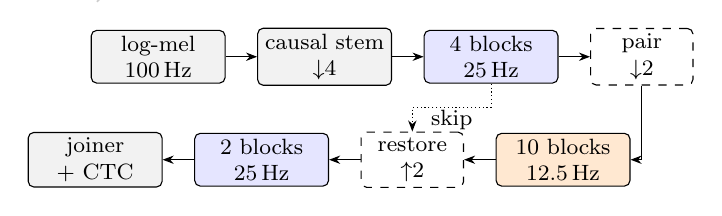
\begin{tikzpicture}[
  font=\footnotesize, >={Stealth[length=4pt]},
  blk/.style={draw, rounded corners=2pt, minimum height=6mm, inner sep=2pt, align=center},
  fast/.style={blk, fill=blue!10, minimum width=17mm},
  slow/.style={blk, fill=orange!18, minimum width=17mm},
  io/.style={blk, fill=gray!10, minimum width=17mm},
  op/.style={blk, fill=white, minimum width=13mm, dashed}]
\node[io] (mel) {log-mel\\100\,Hz};
\node[io, right=4mm of mel] (stem) {causal stem\\$\downarrow$4};
\node[fast, right=4mm of stem] (low) {4 blocks\\25\,Hz};
\node[op, right=4mm of low] (pair) {pair\\$\downarrow$2};
\node[slow, below=6mm of pair, xshift=-10mm] (mid) {10 blocks\\\MidRateHz\,Hz};
\node[op, left=4mm of mid] (rest) {restore\\$\uparrow$2};
\node[fast, left=4mm of rest] (fin) {2 blocks\\25\,Hz};
\node[io, left=4mm of fin] (dec) {joiner\\+ CTC};
\draw[->] (mel) -- (stem); \draw[->] (stem) -- (low); \draw[->] (low) -- (pair);
\draw[->] (pair) |- (mid); \draw[->] (mid) -- (rest); \draw[->] (rest) -- (fin);
\draw[->] (fin) -- (dec);
\draw[->, densely dotted] (low.south) -- ++(0,-3mm) -| node[near start, below, inner sep=1pt]{skip} (rest.north);
\end{tikzpicture}}
\caption{The multirate encoder (S\_MR). Ten of sixteen Conformer blocks run at half rate inside
each 160\,ms chunk; the dense model (S) runs all sixteen at 25\,Hz.}
\label{fig:arch}
\end{figure}

\section{An integer-exact CPU engine}\label{sec:engine}

The engine implements the inference graph in pure Rust, with no ONNX Runtime, BLAS or framework,
its own kernels (scalar reference, AVX2, NEON), and one single-threaded worker per physical core
serving many streams. Every optimisation must leave the output \emph{bit-identical}: hashed
encoder projections and token sequences are the oracle for every kernel change.

\para{Per-row centred INT8.} Weights are quantised per output channel,
$w_q = \mathrm{round}(w/s_w)$ with $s_w=\max|w|/127$. Activations are quantised per
\emph{row}, i.e.\ per frame of one stream, centred on that row's range:
\begin{equation}
\begin{gathered}
c = \tfrac{1}{2}(x_{\max}+x_{\min}),\qquad s_a = \tfrac{1}{254}(x_{\max}-x_{\min}),\\
x_q = \mathrm{rne}\bigl((x-c)/s_a\bigr),
\end{gathered}
\end{equation}
with $|x_q|\le 127$ and round-half-even. The output is recovered exactly as
\begin{equation}
y_{rn} = s_a^{(r)} s_w^{(n)} \textstyle\sum_k x_q w_q \;+\; c^{(r)} \bar w_n + b_n,
\end{equation}
where $\bar w_n = s_w^{(n)}\sum_k w_{q,nk}$ is precomputed, so centring costs one extra fused
multiply-add per output. Centring matters: post-SiLU FFN inputs are one-sided, and an uncentred
symmetric scale wastes half the code range (our first, uncentred attempt cost \IntEightUncentred\pp
WER; centred, the cost on the same set was nil). Because each row's scale and centre come from
that row alone, \emph{a stream's numbers never depend on which streams share its batch}. We
verified this at batch sizes 1, 3, 5, 16 and 32: outputs are bit-identical. This is the property
that dynamic per-tensor INT8, as commonly exported, lacks; in our earlier ONNX export the same
utterance decoded differently alone and in a batch of eight.

\para{Exact integer kernels.} On AVX2 the GEMM tile ($4\times16$) uses \texttt{vpmaddubsw} on
$(|x_q|, \mathrm{sign}(w_q,x_q))$. With both magnitudes at most 127 a pair sums to at most
$2\cdot127^2 = 32{,}258 < 2^{15}$, so the saturating 16-bit step never saturates and the int32
result equals the scalar reference exactly. On ARM the same sums come from \texttt{sdot} and
\texttt{smmla}. Kernel changes that alter a summation order are rejected: an early, faster
attention kernel flipped \AttnFlipCount{} of 400 INT8 transcripts by reordering a float sum, and
was reverted.

\para{Prepared artifacts.} Quantisation happens once, offline. A prepared artifact stores the
packed int8 weights, their scales and column sums, and a manifest with the SHA-256 of the
source weights; the loader verifies both. In qualifying mode the engine refuses runtime weight
quantisation, and every measurement row records the engine configuration, binary hash, commit,
ISA and CPU affinity. Prepared INT8 also lowers peak resident memory for the dense model from
\RssEngineIntEight\,MB (runtime quantisation) to \RssEngineIntEightPrepared\,MB (measured in a
separate run).

\para{Portable log-mel and cross-ISA identity.} Bit-identical kernels are not enough if the
features differ. Our first front end used the platform \texttt{libm} and FMA contraction; the
resulting 1-ULP differences between glibc on x86 and Apple's libm were enough to flip
per-row quantisation ties, and a ternary model decoded \XisaRfourPre{} of 730 utterances
identically across ISAs. We replaced every transcendental with portable, unfused IEEE double
arithmetic (Cody--Waite range reduction with polynomial $\sin$/$\cos$, a mantissa--exponent
polynomial logarithm accurate to half an ULP, precomputed FFT twiddles) and fixed the reduction
order of the AVX2 and scalar paths. Features are now 0-ULP identical across ISAs, and parity with
the PyTorch trainer's features stays below $10^{-6}$ absolute. End to end, from PCM16 to tokens, AVX2 on a
Zen~2 server and NEON on an Apple M3 Ultra agree on \XisaAgree{} of \XisaTotal{} decodes:
\XisaModels{} checkpoints (dense, multirate, int8-stem, ternary) $\times$ FP32 and INT8 $\times$ the
730-utterance panel (\cref{tab:xisa}).
Exactness did not cost speed in the front end: a sparse triangular filterbank
(\MelNnzSparse{} instead of \MelNnzDense{} nonzero weights), precomputed bit reversal and an
unfused vectorised double-precision FFT (four lanes on AVX2, two on NEON) make log-mel
\MelSpeedupZen{}$\times$ faster on Zen~2 and \MelSpeedupMthree{}$\times$ on M3 while staying 0-ULP
identical to the portable reference.

\para{Where the time goes.} At a single stream on Zen~2 the int8 GEMMs take \GemmShare\% of engine
time, at about \GmacPerCore{} GMAC/s per core; attention is the largest remaining phase, and the
greedy decoder costs about \GreedyDecoderCost{} \cpus. At batch the engine is compute-bound:
sixteen streams per worker lower CPU per stream by at most \BatchLift\%, which shapes both the
density result and the negative results of \cref{sec:negative}.

\section{Training}\label{sec:training}

\para{Data and pseudo-labelling.} \ultra{} is trained on
LibriSpeech~\cite{panayotov2015librispeech} 960\,h combined with Libri-Light~\cite{kahn2020librilight}
pseudo-labelled by the pretrained streaming Zipformer INT8 model (R0, also the Zipformer comparator
in \cref{fig:money,tab:measured}), so its pseudo-labels inherit the Zipformer teacher's domain and
text style. Training logged \CandTrainKh\,h of audio: LibriSpeech until live WER saturates, then
Libri-Light (small, medium, large) and an EMA cooldown. In our runs LibriSpeech alone plateaus while new
audio keeps lowering WER, so for a model this small the lever is data diversity, not epochs.

\para{Recipe.} We optimise the joint RNN-T and auxiliary CTC loss (CTC weight \CtcWeight) with
AdamW, cosine learning-rate decay, SpecAugment~\cite{park2019specaugment}, speed perturbation, and
a small emission delay penalty (\DelayPenalty) to keep live-stream word latency low. The RNN-T loss
evaluates the joiner in time chunks without materialising the full $(B,T,U{+}1,V{+}1)$ lattice.
Training finishes with an exponential moving average (EMA)~\cite{polyak1992ema} cooldown phase,
yielding a single checkpoint whose weights are exported to prepared per-channel INT8 with zero
quantisation-aware retraining. The 5-gram language model (\texttt{M5.ulm}) used in the
utterance-segmented commit pass is trained on the standard LibriSpeech OpenSLR-11 text corpus.

\section{Evaluation Protocol}\label{sec:protocol}

\para{Workload and scoring.} Every system in \cref{fig:money,tab:measured} decodes the exact same
staged audio: a 730-utterance LibriSpeech DEV panel (\ColdAudioMinutes\,min; 400 dev-clean utterances
from 40 speakers and 330 dev-other utterances from 33 speakers, covering every DEV speaker). A single
Rust scorer (\texttt{ultra-score}) and text normaliser score every hypothesis. WER pools edits and
reference words over the utterance population $U$:
\begin{equation}
\mathrm{WER}(U)=100\,\frac{\sum_{i\in U}(S_i+D_i+I_i)}{\sum_{i\in U}N_i}.
\end{equation}
We report dev-clean, dev-other, and pooled panel WER for every system, plus full LibriSpeech DEV
(\RelFullUtts{} utterances) accuracy for \ultra{}.

\para{Timing hosts and classes.} Each run uses one process with one inference thread pinned to one
physical Zen~2 core, alone on its 4-core L3 complex. We report the median over three cold runs of
CPU-seconds per audio-second (\cpus) and its reciprocal, throughput in $\times$ real time, with peak
resident memory (RSS) and artifact size. Primary rows are measured on the otherwise idle host H1
(AMD Threadripper PRO 3995WX, 4 of 8 memory channels; at most two other busy cores, host timers and CI
paused). Rows measured earlier on the shared host H0 (same CPU, 2 of 8 channels) are marked interim. Systems are \emph{live streaming} (words emitted continuously, no endpoint),
\emph{streaming + utterance-segmented commit} (\ultra{} final), or \emph{offline whole-utterance}
(Parakeet TDT v3, drawn hollow in \cref{fig:money}).

\para{Energy.} On H1, CPU energy is read from the service core's RAPL energy register during the
timing run and divided by decoded audio seconds (core domain only, not wall power); peak RSS is that of the recogniser process tree ($10^6$ bytes). The interleaved R6
rows (\ultra{} and Zipformer INT8) subtract the core idle floor (a versioned energy-bench record).
Separately timed Moonshine, Parakeet, and Nemotron joins include that floor, so their joules are not a
paired ratio against the R6 rows.

\para{Test-set disclosure and INT8 gate.} All accuracy numbers are LibriSpeech DEV only. Following our
benchmark freeze protocol, LibriSpeech test-clean and test-other were read several times before the
freeze, and no checkpoint selection used test data. Prepared INT8 artifacts must pass a paired
speaker-cluster bootstrap~\cite{bisani2004bootstrap} gate against FP32 within \PreregDeltaPP\pp point
delta and \PreregUpperPP\pp one-sided 95\% upper bound.

\section{Results}\label{sec:results}

\subsection{All Public CPU Comparators vs.\ \ultra{}}\label{sec:compare}

\Cref{fig:money} and \cref{tab:measured} place \ultra{} live beside every timed public
open-weights CPU comparator. \ColdHostSentence{} \ColdSubsetSentence{}

\para{Speed and power.} On one quiet Zen~2 core, \ultra{} live decodes cold at \ColdLiveSpeed$\times$
real time (\ColdLiveRss\,MB peak memory) at \ColdLiveWer\% pooled panel WER; \ultra{} final runs at
\ColdHeadSpeed$\times$. \ColdMemorySentence{} In the paired R8 full-panel blocks, live is
\ColdLiveWatts\,J per audio-second, \VsEnergyPctOne\% of the Zipformer INT8 anchor timed in the same blocks (R6 row:
\ColdZipRsixWatts\,J); in the paired R9 blocks (same protocol and anchors), the v4.2.0 final pass is \ColdHeadWatts\,J. The R7 matched campaign, which idle-subtracts every plotted comparator,
puts Zipformer INT8 at \RsevenZipEnergy\,J on its \RsevenClips-clip subset. At utterance
endpoints the commit pass runs at \ColdFinalCorePct\% of one core (\ColdFinalVsZipSpeed).

\para{Accuracy.} The utterance-end \ultra{} final pass on its own weights reaches \ColdHeadWer\% pooled panel
WER (\FinPanelClean\% dev-clean, \FinPanelOther\% dev-other), \VsVerdictTwo{} streaming Zipformer INT8's \ColdZipWer\%
(\FinPanelZipClean\% dev-clean) under the paired test below, and is the lowest measured dev-clean WER among timed
CPU recognisers at $\geq 14\times$ real time (full-DEV clean \FinFullClean\% vs.\ Zipformer \FinFullZipClean\%).
\ultra{} is trained on Libri-Light pseudo-labels from that Zipformer (R0). Larger 600M-parameter models
achieve lower WER at much higher CPU cost and, where metered, higher energy; they are not in the $\geq 14\times$ group.

\subsection{Head-to-Head with Zipformer INT8 and Full-DEV Accuracy}\label{sec:versus}

Zipformer INT8 is the strongest public streaming comparator near our cost point and the teacher of our
pseudo-labels, so we compare against it directly on the same utterances and core (\cref{tab:versus}),
timed in the same three interleaved blocks on quiet H1 (R8 for live, R9 for the v4.2.0 final pass); speed, energy and memory ratios are medians of
within-block ratios, and WER differences are paired with speaker-cluster bootstrap. Because the
730-utterance panel overlaps the selection half of DEV, we also report the unselected confirmation half
(C, \LookCUtts{} utterances), decoded once for each frozen release: there, \ultra{} live is \LookLiveCZipDelta\pp from
Zipformer (bounds \LookLiveCZipLo{} to \LookLiveCZipHi), not a significant difference. \ultra{} live uses \VsCpuPctOne\% of Zipformer's CPU time
(\VsSpeedXOne$\times$ throughput), \VsEnergyPctOne\% of its active core energy (paired R8 blocks), and \VsRssPctOne\% of its
memory with half the chunk (\VsChunkOne\,ms vs.\ \VsZipChunk\,ms); its panel WER is \VsVerdictOne{}
Zipformer's (\VsDeltaOne\pp, bounds \VsLoOne{} to \VsHiOne\pp). \ultra{} final is \VsVerdictTwo{}
Zipformer's (\VsDeltaTwo\pp, bounds \VsLoTwo{} to \VsHiTwo\pp; lower on C at \FinCZipDelta\pp, bounds \FinCZipLo{} to \FinCZipHi) at
\VsSpeedXTwo$\times$ its single-core speed and \VsEnergyPctTwo\% of its active core energy.

\para{What v4.2.0 changes.} Only the final pass changed. Against the v4.1.0 final pass on the same utterances,
v4.2.0 final is \FinPanelPrevDelta\pp on the panel (bounds \FinPanelPrevLo{} to \FinPanelPrevHi), \FinCPrevDelta\pp on
the unselected C half (bounds \FinCPrevLo{} to \FinCPrevHi; dev-clean \FinPrevCClean\% $\to$ \FinCClean\%), and the gated beam-48
re-search alone is \FinSBaseDelta\pp on the selection half against the same pass without it (bounds \FinSBaseLo{} to
\FinSBaseHi). In the paired R9 blocks the whole pass changes CPU time per audio-second by \FinCostCpuPct\% and core
energy by \FinCostEnergyPct\% against the released v4.1.0 final binary; the gate alone costs \FinGateCpuPct\% CPU and
\FinGateEnergyPct\% energy against the same build with the gate off, at the +\FinGateBudgetPct\% budget set for it (locked by owner choice when
research timing put it just over).

On full LibriSpeech DEV (\RelFullUtts{} utterances, which contains the selection half and is therefore
descriptive), \ultra{} live reaches \LookLiveFullClean\% dev-clean, \LookLiveFullOther\% dev-other
and \LookLiveFullWer\% pooled WER; \ultra{} final reaches \FinFullClean\% dev-clean, \FinFullOther\% dev-other and
\FinFullWer\% pooled (v4.1.0 final: \LookFinalFullWer\%).

\begin{table}[t]
\centering
\caption{\textbf{Head-to-head with Zipformer INT8}: same 730 DEV utterances (the selection panel; the unselected-half gaps are in \cref{sec:versus}), same quiet Zen~2 core, same interleaved blocks, median of three. Ratios are medians of within-block ratios. $\Delta$ is paired (speaker-cluster bootstrap); negative means fewer errors. Cell colour: green is better, red worse.}
\label{tab:versus}
\footnotesize
\setlength{\tabcolsep}{1.5pt}
\begin{tabular}{@{}lrr@{}}
\toprule
Metric & Zipformer & \ultra{} live \\
\midrule
Live chunk (ms) & 320 & 160 \\
Pooled WER (\%) & \hmcell{A7F3D0}{5.25} & \hmcell{FECACA}{5.54} \\
$\Delta$ WER vs.\ Zip.\ (pp) & --- & +0.28 \\
\quad one-sided 95\% bounds & --- & [$-$0.02, +0.58] \\
1-core speed ($\times$ RT) & \hmcell{FECACA}{14.0} & \hmcell{A7F3D0}{32.7} \\
J per audio-s (core) & \hmcell{FECACA}{0.573} & \hmcell{A7F3D0}{0.328} \\
Peak RSS (MB) & \hmcell{FECACA}{152} & \hmcell{A7F3D0}{109} \\
\bottomrule
\end{tabular}
\end{table}


\section{Negative results}\label{sec:negative}

\para{Ternary weights that fit in L3 are not faster at batch.} We trained the multirate model with
ternary weights $\{-1,0,+1\}$ and per-channel absmean scales by quantisation-aware fine-tuning
from a 100\,h checkpoint~\cite{ma2024bitnet}, with activations fake-quantised exactly as the
engine quantises them. The ternary model costs \TernaryWerCost\pp WER and stores its encoder in
\TernaryMiB\,MiB, which fits a Zen~2 CCX's 16\,MiB L3. The engine's ternary lookup kernel wins at a
single stream, where weight traffic dominates. At batch it loses: \TernaryDenCCX{} streams per CCX
against \IntEightMRDenCCX{} for INT8 multirate on x86, both measured with the engine's development
tool (not the evaluation harness, so not comparable with \cref{tab:density}). Once sixteen or more streams share each weight traversal
the engine is compute-bound, weight bytes stop mattering, and the int8 dot-product units do more
useful work per cycle than table lookups.

\para{Removing instructions does not remove time.} On AVX2 the signed int8 GEMM spends three of
ten instructions per 64 multiply-accumulates on taking absolute values and transferring signs. An
unsigned-offset 7-bit tile removes all three and is bit-exact against our 7-bit reference. On Zen~2 it is
\emph{slower}: \UsevenVsKzeroLo--\UsevenVsKzeroHi{}$\times$ the speed of the signed tile across
layer shapes and hosts, against a pre-registered bar of \UsevenBar$\times$. It keeps four vector
multiplies per 64 MACs; the 7-bit activation variant, which drops one multiply, is the only one that
wins, by about \ActSevenGain\%. On this core time per MAC follows the multiply count, not the
instruction count.

\para{Bit-identical non-GEMM cuts are small.} Hoisting rotary tables and fusing residual adds
with the next normalisation are bit-identical and kept, but gain only \NonGemmGain\% end to end,
inside run-to-run noise: the remaining non-GEMM time is real attention work, not overhead.

\section{Limitations}\label{sec:limitations}

\para{Utterance-segmented final mode and memory.} \ColdLimitLive{} Shrinking LM memory
(\LmPackMb\,MB on disk) and commit CPU without losing accuracy is active work.

\para{Live accuracy.} The endpoint-free live stream trades accuracy for cost: its gap to Zipformer INT8 is \CandLiveLmCDelta\pp on the unselected half of DEV (\cref{sec:candidate,sec:v4negative}), so applications that need Zipformer-class text before an utterance ends should not assume the final-pass accuracy.

\para{Training data and LM overlap.} \ultra{} \ReleaseVer{} is trained on LibriSpeech 960\,h plus
Libri-Light pseudo-labelled by R0 (the Zipformer comparator). Release comparisons use read English
LibriSpeech DEV audio, which is in-domain for both \ultra{} and Zipformer; rankings on
conversational, accented, or noisy speech may differ. The OpenSLR-11 training text of
\texttt{M5.ulm} contains \LmOverlapCount{} of the \LmOverlapOf{} longer DEV transcripts verbatim;
removing them leaves the relative LM WER gain unchanged.

\para{Host coverage, energy scope, and DEV-only claims.} \ColdHostSentence{} \ColdSubsetSentence{}
Shared-host (H0) rows stay marked interim until quiet H1 holds complete. Energy measurements are
active core (CPU-domain) joules per audio-second from RAPL registers (\texttt{core\_msr\_active}, including
the core idle floor; package domain was measured only for the prior release), never board or wall power, and are
measured unpaced for apples-to-apples comparison across recognisers. All accuracy numbers are LibriSpeech DEV only; as disclosed in
\cref{sec:protocol}, LibriSpeech test-clean and test-other were read several times before our
benchmark freeze, and no test-set numbers appear here.

\section{Conclusion}\label{sec:conclusion}

An always-on speech recogniser should barely register on the CPU budget of the machine hosting it.
We presented \ultra{} \ReleaseVer{}, a compact streaming Conformer transducer and pure-Rust
integer-exact CPU engine evaluated against all \ColdCompleteCompCount{} complete-panel public
open-weights CPU comparators on the same 730-utterance LibriSpeech DEV panel. On one pinned quiet
Zen~2 core and one prepared INT8 artifact, \ultra{} \ReleaseVer{} delivers \ColdConclusionResult{},
reproduces its transcripts exactly on \CandIsaRuns{} witness decodes across x86 and ARM CPUs; the
prior release sustained sixteen real-time paced live streams at \RelCapSixteenBusy\% of one core
(\RelCapSixteenNetW\,W net per stream, \RelCapSixteenLagPninetyFive\,ms p95 lag) with INT8 execution within
\RelIntEightDelta\pp of FP32. \ultra{} \ReleaseVer{} is released by owner decision: it missed its registered
full-DEV final gate (\CandFinalFullEdits{} edits against \CandGateFinalFull) and trails Zipformer by
\CandLiveLmCDelta{} points on the unselected half of DEV for the live stream with a language model.
All results are exploratory and use development data only. The negative results of \cref{sec:v4negative} point to the next lever: more acoustic evidence, that is fresh audio rather than relabelled audio, and capacity paid for by the power savings.


\bibliographystyle{IEEEtran}
\bibliography{refs}

\end{document}
